%!TEX root = ../Thesis.tex
\section{Introduction}
\label{sec:introduction}
The \gls{IMF} is an organization comprised of 189 countries and established in 1944. Its goal is to foster cooperation in trade between its members and secure their and the global financial stability. The \gls{IMF} has three main functions: economic surveillance, financial assistance and capacity development.

\begin{figure}[hbt]
\centering
\begin{minipage}[t]{.7\textwidth} % Breite, z.B. 1\textwidth		
\caption{International Monetary Fund Organization Chart} % Überschrift
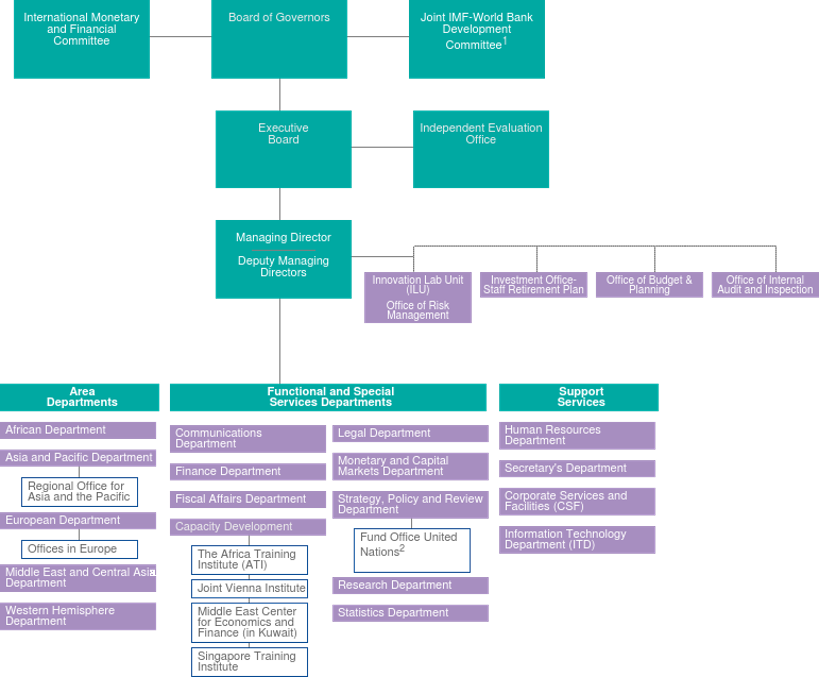
\includegraphics[width=1\textwidth]{img/orgchart}\\ % Pfad
\source{https://www.imf.org/external/np/obp/orgcht.htm} % Quelle
\label{fig:orgchart}
\end{minipage}
\end{figure}